\begin{figure}[H]
\begin{subfigure}[t]{0.45\linewidth}
    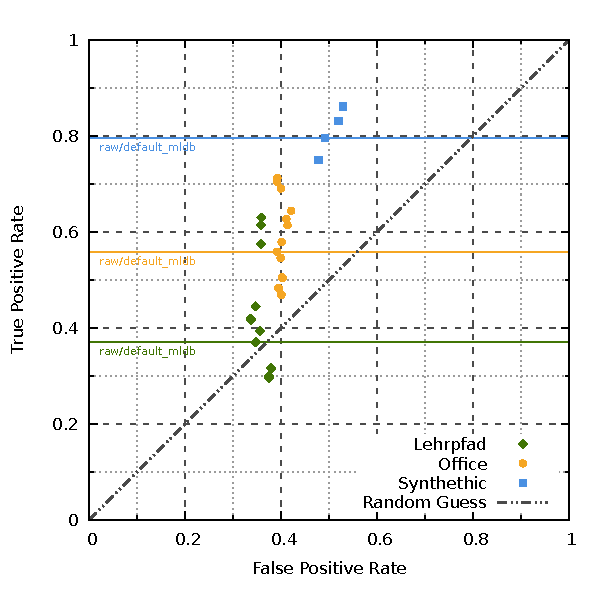
\includegraphics[width=\linewidth]{chapter06/results/AKAZE/flexion/roc.pdf}%
    \caption{Flexion Image ROC}
\end{subfigure}\quad
\begin{subfigure}[t]{0.45\linewidth}
    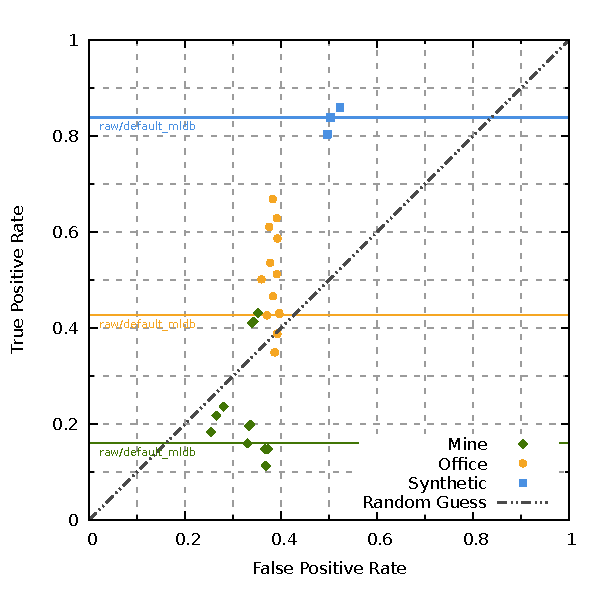
\includegraphics[width=\linewidth]{chapter06/results/AKAZE/bearing/roc.pdf}
    \caption{Bearing-Angle Image ROC}
\end{subfigure}
    \caption{AKAZE}
\end{figure}

\begin{figure}[H]
\begin{subfigure}[t]{0.45\linewidth}
    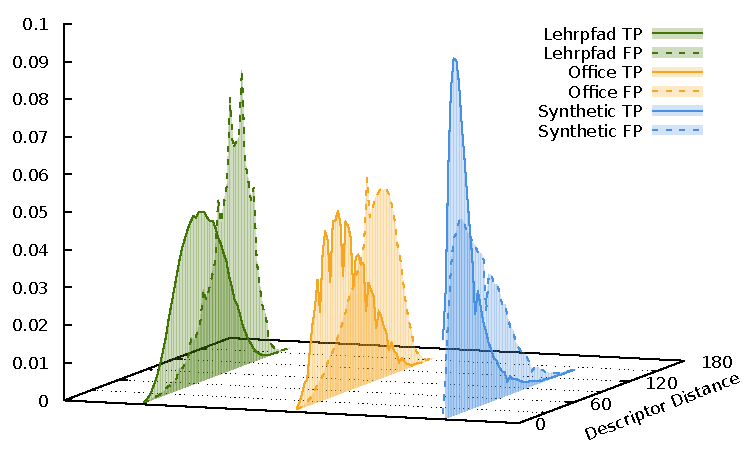
\includegraphics[width=\linewidth]{chapter06/results/AKAZE/flexion/descriptor_distances.pdf}%
    \caption{\gls{flexion-image} Descriptor Distances}
\end{subfigure}\quad
\begin{subfigure}[t]{0.45\linewidth}
    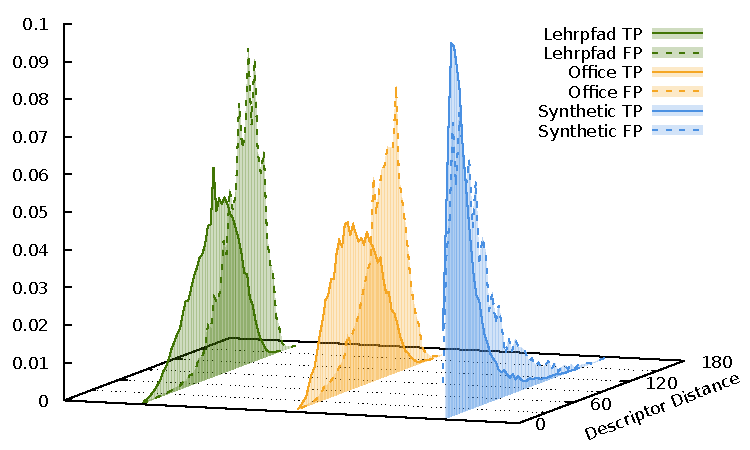
\includegraphics[width=\linewidth]{chapter06/results/AKAZE/bearing/descriptor_distances.pdf}%
    \caption{\gls{bearing-angle-image} Descriptors Distances}
\end{subfigure}
\end{figure}
